% Chap2_sota.tex
\chapter*{State of the Art}

\section*{Batteryless technology}
        
    \paragraph{}
        The usage of batteries contributes significantly to both environmental concerns (battery waste) and economic issues due to their short lifespans, necessitating frequent replacements even for rechargeable variants. The demand for battery-free alternatives has been steadily increasing, particularly across various domains such as machine learning, activity recognition, and greenhouse monitorings%\cite{sourceOfArticle}. 

    \paragraph{}
        Let's begin with a fundamental example that is commonly encountered in our daily lives: credit cards equipped with \gls{rfid} chips.
        \newline
        These chips employ a remarkable energy-harvesting technique, drawing electromagnetic energy from the reading device itself and responding to the \textit{Read} query (Upper section of figure \ref{fig:energy-harvestingRFiD}). This innovative approach obviates the requirement for a consistent energy supply. As a result, it enables the creation of incredibly compact designs that can seamlessly integrate into a wide array of environments, including the human body.

    \paragraph{}
        Advanced modes of operation are also achievable, utilizing harvested energy to perform computations via \gls{crfid}. Revisiting our earlier example, we can envision a device that captures the temperature sensor's output and stores it in \gls{nonVolatileMemory} when subjected to an electromagnetic field associated with a specific query (Lower section of figure \ref{fig:energy-harvestingRFiD}) with a specific power.
        Depending of the power injected into that electromagnetic field, the device will in capacity or not to compute the task\cite{rfidEnergyAwareCheckpointing}.
    
    \begin{figure}[htbp]
        \centering
        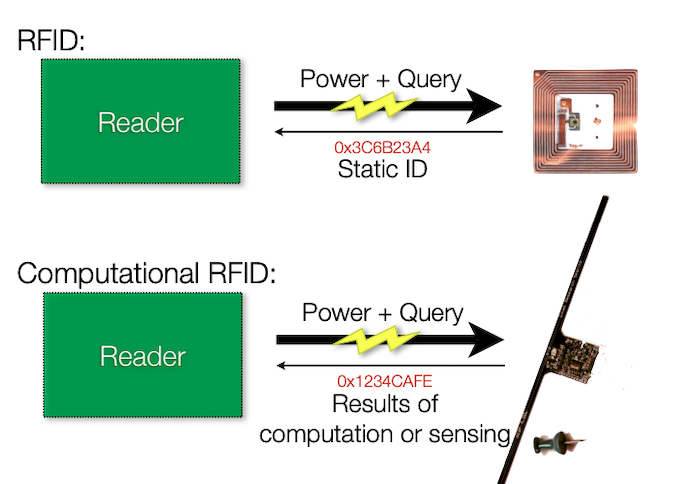
\includegraphics[width=0.6\textwidth]{img/chap2/Diagram_of_the_difference_between_RFID_and_computational_RFID.jpg}
        \caption{Illustration of difference between \gls{rfid} and \gls{crfid}\cite{presentationRfidEnergyAwareCheckpointing}, Slide 14.}
        \label{fig:energy-harvestingRFiD}
    \end{figure}

    \paragraph{}
        Having explored individual applications, let's now envision the vast possibilities offered by a family of distributed sensor network systems. This visionary concept has been set in motion by projects like \gls{smartdust} and \gls{terraswam}, which seek to create a network of minuscule sensors (each measuring just 1 mm in size) with the ability to collectively establish distributed sensor network systems.
    
    \paragraph{}
        The core idea of these projects is \gls{ciot}, involves deploying a multitude of sensors that can collaborate to collect data, communicate seamlessly, and process information collectively. This interconnected web of diminutive sensors holds transformative potential across numerous domains, spanning environmental monitoring, disaster response, healthcare, and industrial automation. The capabilities of such systems transcend the scope of individual applications, introducing novel dimensions of data acquisition, analysis, and responsiveness\cite{colloborativeIoT}.
    
    \paragraph{}
        In this introduction, we briefly grasp the purpose of utilizing \gls{batteryless} devices and explore the potential of their applications. While we've discussed one energy source involving electromagnetic fields, other sources like solar, wind, or thermal energy are equally viable options. The primary challenge of employing such devices lies in Energy Harvesting, a topic that will guide us to the subsequent section.
    

    
\section{Energy Harvesting Mechanisms}
    In a \gls{batteryless} context, Energy Harvesting has been recognized as inherently non-consistent. As devices lack a stable power supply, it falls upon the device's hardware and software to manage this variability.

    \paragraph{}
        Illustrated in this example (Figure \ref{fig:energy-harvesting}), you can observe the charging lifecycle of a device's stored energy (capacitor) alongside its execution time. Depending on the frequency of charging, it becomes evident that without suitable adaptation of the device's behavior, the consistency of received data deteriorates. Notably, the transmission of messages occurs only when all required data is collected. This strategy necessitates minimal processing and energy consumption for data storage.

    \begin{figure}[htbp]
        \centering
        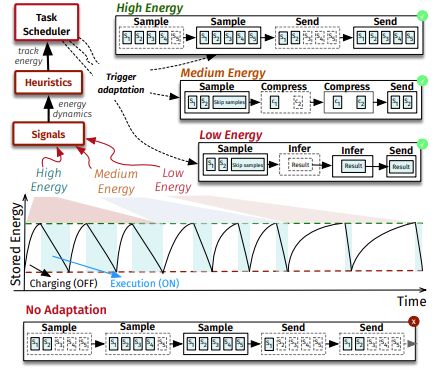
\includegraphics[width=1\textwidth]{img/chap2/Figure - simple sense and send application .png}
        \caption{A simple sense and send application samples the temperature sensor 5 times and sends it to a base station.Energy harvesting causes power scarcity and outages creating a non-termination state. Checkpoints or task divisions maintain forward progress but lead to a greedy execution that takes a much longer time. Adaptive execution strategies (top of the figure) quickly adapt to changing environmental conditions and finish o! quickly—using harvested energy efficiently by gracefully modifying execution.\cite{basedArticle}.}
        \label{fig:energy-harvesting}
    \end{figure}

    \paragraph{}
        As depicted in the figure \ref{fig:energy-harvesting}), several options are already available for adapting the strategy to be employed. This forms the subject of our upcoming section on Challenges of Intermittency.
    

\newpage

\section{Challenges of Intermittency}
    In this section, we will delve into the challenges posed by intermittency and analyze the current state of research. The primary concern lies in maintaining operational continuity and ensuring the quality of data delivery. In cases of task failure due to power outage, data can be compromised through data loss, corruption, or reliance on outdated information. Addressing these concerns involves implementing certain mechanisms\cite{basedArticle}\cite{rfidEnergyAwareCheckpointing}:

    \begin{itemize}
        \item Introducing checkpoints within the program code: involves storing the current state of information in \gls{nonVolatileMemory}, such as \gls{fram}\footnote{FRAM is commonly employed in the IoT domain due to its lower power consumption in comparison to conventional storage devices like flash drives\cite{enwiki:1169326001}.}. When a power outage occurs, the state is preserved. Once energy harvesting is available, the task can resume from its previous state and continue until the next power interruption or the completion of the process.
        \item \gls{atomizeprocesses} by creating task-based structures: This method employs \gls{allornothingsemantics}, with tasks committed to \gls{nonVolatileMemory} upon completion.
    \end{itemize}

    \paragraph{}
        Another approach involves opting for a computing pattern. As depicted in Figure \ref{fig:energyadaptivestrategies}, various strategies are available. In the diagram, Strategy One involves initially collecting a certain amount of data before proceeding to computation. In contrast, Strategy Two entails computing each collected data sample individually\cite{10.1145/3478077}.

        
    \begin{figure}[htbp]
        \centering
        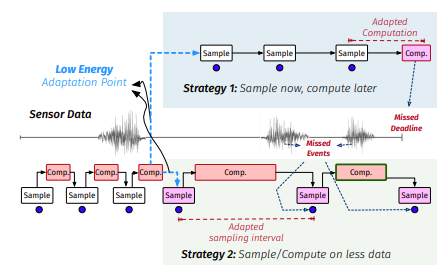
\includegraphics[width=1\textwidth]{img/chap2/Figure - different strategies.png}
        \caption{For an activity recognition application, two different adaptation strategies are shown: one that prefers gathering samples consistently and waiting to  compute over them, and another that gathers fewer samples and computes on them. In strategy 1; deadlines may be missed since no inference is done, but events are all captured, in strategy 2; sampling is reduced to meet the deadlines, but events may be missed. While both strategies are likely better than not adapting, the choice of how to adapt greatly depends on the application programmers goals.\cite{10.1145/3478077}}
        \label{fig:energyadaptivestrategies}
    \end{figure}

    \paragraph{}
        These approaches \textit{can} be effective for short periods of power loss. However, as the duration of power outages increases, so does the risk of generating irrelevant output (outdated, inconsistent, or nonexistent data) and wasting energy on storing such data\cite{basedArticle}.



    \paragraph{}
        The challenges posed by intermittency have been under exploration since at least the early 1990s\cite{259428}. One notable response to this challenge can be observed in the adaptation of smartphones running on Android\cite{10.5555/2813767.2813810}. When the battery level becomes lower, various adjustments are made such as software downgrades, limiting screen brightness, or reducing the screen's frequency rate\cite{basedArticle}.

    \newpage
    \subsection{When to Adapt}
        Two approaches are presented, yet neither covers all scenarios\cite{basedArticle}:
        \begin{itemize}
            \item Identifying a general method to predict power outages: This method is challenging to generalize due to the diversity of energy harvesting modes and trends (e.g., diurnal shifts, activity based on kinetic harvesting, etc.) and the variety of devices involved.
            \item Implementing a task to record and analyze trends at runtime: This approach demands significant energy, space, and time resources.
        \end{itemize}
        
        \noindent
        However, neither of these approaches is completely resilient to power outages, which can ultimately lead to inconsistencies.
        

    \subsection{What to Adapt}
        When addressing the question of "What" to adapt, the focus typically revolves around enhancing or degrading performance based on energy availability.
        
        \paragraph{}
        This availability can be partially managed by adjusting behavior. However, it's up to the developer, as previously mentioned, to implement a task that estimates the available energy and adjusts the scheme according to the Energy Mode (refer to Figure \ref{fig:energy-harvesting}). For instance, an application could have an energy task (to implement) which returns the energy mode and adapts its processing accordingly\ref{table:energymode}:
        
        \begin{table}[h]
        \centering
        \begin{tabular}{|c|c|}
        \hline
        \textbf{Energy Mode} & \textbf{Processing Sequence} \\
        \hline
        High & SENSE -> COMPUTE -> SEND, or SENSE -> SEND \\
        Medium & SENSE -> FILTER -> SEND \\
        Low & SENSE -> INFER -> SEND \\
        \hline
        \end{tabular}
        \caption{Adapted Strategies Based on Energy Mode}
        \label{table:energymode}
        \end{table}
        
        \noindent
        However, this approach is quite specific, and providing a general framework to make decisions about fatigue, priority, and the selection of valuable samples remains a considerable challenge\cite{basedArticle}.

    \paragraph{}
        Before concluding this section, let's highlight the primary research question that has been identified: 'How can energy intermittency be effectively managed in batteryless devices?'

    \paragraph{}
        As we have observed, existing research can address certain scenarios. However, for prolonged power disruptions, determining the appropriate course of action becomes complex and requires flexibility through adaptive mechanisms. This brings us to the next section, where we will explore the \gls{heuristic} Adaptation.

\newpage
\section{Proposed Heuristic Adaptation Technique}
        In response to these challenges, the authors introduced the \gls{rehash} framework. Its key feature is the implementation of \gls{heuristic} adaptation, a result of intermittent execution due to energy arrivals and varying energy availability\cite{basedArticle}. This framework is designed to streamline the development of adaptive solutions by introducing a \gls{heuristic} function that estimates energy availability within the environment with minimal overhead.
        
    \paragraph{}
    The design goals and features of \gls{rehash}\ref{fig:REHASH} for intermittent systems encompass four elements:
    \begin{itemize}
        \item Portable Energy Approximation: Heuristic adaptation establishes a standardized approach for estimating available energy and making informed adaptation decisions.
        \item Multiple Signals: Various signals, such as minimum, maximum, or average values, can trigger adaptation decisions.
        \item Versatility in Adjustment: A range of parameters, including sampling rates, transmit power, neural network depth, etc., can be adjusted for adaptation.
        \item Flexible and Fine-Grained Adaptation Constructs and Strategies: Developers can anticipate worst-case scenarios and dictate the "when," "what," and "how" of adaptation. This empowers developers to tailor adaptation strategies for specific applications.
    \end{itemize}
    
    \begin{figure}[htbp]
        \centering
        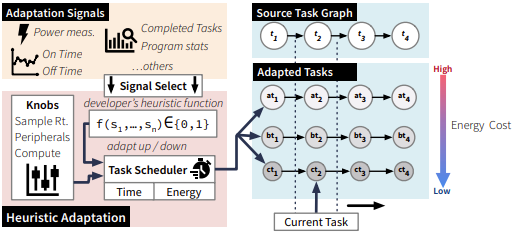
\includegraphics[width=1\textwidth]{img/chap2/Figure - REHASH.png}
        \caption{Overview of our REHASH framework for heuristic adaptation. The hardware measures signals of the state of the energy harvesting environment such as on-time, o!-time, task count, and recent events. A developer-defined heuristic function takes these signals in a logic equation that decides whether to adapt up (increasing energy use) or degrade performance (decrease energy use). The heuristic function embodies the developers application goals. The next adapted task replica is chosen, while the task scheduler obliviously executes the next (adapted) task.\cite{10.1145/3478077}}
        \label{fig:REHASH}
    \end{figure}

    \paragraph{}
    The tracking of the energy dynamics is possible by listen the time interval length from the time the capacitor is fully charged until the system failed which can be exploited as an adaptation signal\ref{fig:REHASHsignal}.
    \begin{itemize}
        \item On-Time: Measure the Uncharge (Execution) time of the capacitor from fully loaded until the device failed
        \item Off-Time: Measure the Charge time of the empty capacitor
        \item Task Count: Measure the count of task completed to estimate if it's remained more energy available.
    \end{itemize}

    \paragraph{}
        Tracking energy dynamics can be achieved by observing the length of time intervals from when the capacitor is fully charged to the point of system failure. This interval can serve as an exploitable adaptation signal\ref{fig:REHASHsignal}. There are three key signals that can be utilized:
        
    \begin{itemize}
        \item On-Time: Measure the execution time of the capacitor from full charge until device failure.
        \item Off-Time: Measure the charging time of the empty capacitor.
        \item Task Count: Count the completed tasks to estimate if there is remaining available energy.
    \end{itemize}

    \begin{figure}[htbp]
        \centering
        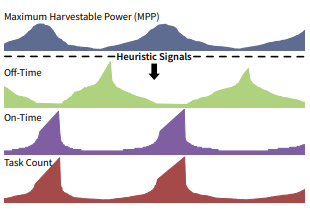
\includegraphics[width=0.6\textwidth]{img/chap2/Figure - REHASH Signals.png}
        \caption{This figure shows that signals in our framework track the maximum power harvestable from an energy environment, providing a useful estimate of energy availability trends. The signal values are drawn from an execution of the MNIST machine learning application on the energy environment.\cite{10.1145/3478077}}
        \label{fig:REHASHsignal}
    \end{figure}

    \paragraph{}
        Returning to the central challenge of determining "When," "How," and "What" actions should be taken, the \gls{rehash} framework offers a solution that addresses these aspects\cite{basedArticle}. The coverage provided by the framework can be understood as follows:
        
        \begin{itemize}
            \item \textbf{When:} This aspect is addressed by the \gls{heuristic} function, which dynamically adapts parameters based on the situation.
            \item \textbf{What:} The framework covers this by providing Knobs, which are APIs enabling developers to design adapted routines. Additionally, a simulation tool is proposed.
            \item \textbf{How:} The \gls{heuristic} function identifies whether adaptation should go up or down, while the Knobs facilitate the creation of routines.
        \end{itemize}